\documentclass[referat]{SCWorks}

\usepackage{preamble}

\begin{document}

% Кафедра (в родительном падеже)
\chair{информатики и программирования}

% Тема работы
\title{Компьютерная графика и её реализация на C++}

% Курс
\course{1}

% Группа
\group{111}

% Специальность/направление код - наименование
\napravlenie{02.03.02 "--- Фундаментальная информатика и информационные технологии}

\department{факультета Компьютерных наук и информационных технологий}

\studenttitle{студентов}

% Фамилия, имя, отчество в родительном падеже
\author{Алексеева Никиты Игоревича \\ Зинченко Елены Валентиновны \\ Неклюдовой Марины Сергеевны}

% Научный руководитель (для реферата преподаватель проверяющий работу)
\satitle{доцент, к.\,п.\,н.} % должность, степень, звание
\saname{А.\,П.\,Грецова}

% Год выполнения отчета
\date{2025}

\maketitle

% Включение нумерации рисунков, формул и таблиц по разделам (по умолчанию -
% нумерация сквозная) (допускается оба вида нумерации)
\secNumbering

\tableofcontents

\intro
Представление данных на мониторе компьютера в графическом виде впервые было реализовано в середине 50"=х годов для больших ЭВМ, применявшихся в научных и военных исследованиях. С тех пор графический способ отображения данных стал неотъемлемой принадлежностью большинства компьютерных систем, в особенности персональных. Графический интерфейс пользователя сегодня является стандартом \flqq де"=факто\frqq\ для программного обеспечения разных классов, начиная с операционных систем.

Существует специальная область информатики, изучающая методы и средства создания и обработки изображений с помощью программно"=аппаратных вычислительных комплексов "--- компьютерная графика. Она охватывает все виды и формы представления изображений, доступных для восприятия человеком либо на экране монитора, либо в виде копии на внешнем носителе (бумага, кинопленка, ткань и прочее). Без компьютерной графики невозможно представить себе не только компьютерный, но и обычный, вполне материальный мир. Визуализация данных находит применение в самых разных сферах человеческой деятельности. Для примера назовем бизнес и экономику, медицину (компьютерная томография), научные исследования (визуализация строения вещества, векторных полей и других данных), моделирование тканей и одежды, опытно"=конструкторские разработки.

Хотя компьютерная графика служит всего лишь инструментом, ее структура и методы основаны на передовых достижениях фундаментальных и прикладных наук: математики, физики, химии, биологии, статистики, программирования и множества других. Это замечание справедливо как для программных, так и для аппаратных средств создания и обработки изображений на компьютере. Поэтому компьютерная графика является одной из наиболее бурно развивающихся отраслей информатики и во многих случаях выступает \flqq локомотивом\frqq\, тянущим за собой всю компьютерную индустрию.

\section{Основы компьютерной графики}
\subsection{Введение в компьютерную графику}
\textbf{Компьютерная графика} "--- это область науки и технологии, связанная с созданием, обработкой и отображением изображений с помощью компьютера. Цель компьютерной графики "--- создание и обработка изображений с помощью компьютеров и программного обеспечения для решения различных задач в разных областях.

Основные задачи:
\begin{enumerate}
    \item Создание и редактирование изображений. Разработка инструментов и методов для изменения графических изображений.  
    \item Визуализация данных. Преобразование данных в визуальные формы для более лёгкого понимания и анализа.  
    \item Анимация и моделирование. Создание движущихся изображений и трёхмерных моделей для различных приложений.  
    \item Интерактивность. Разработка графических интерфейсов, которые позволяют пользователям взаимодействовать с изображениями и данными.  
    \item Фотореалистичность. Достижение максимальной реалистичности в изображениях, чтобы они выглядели как реальные фотографии или натурные сцены.
\end{enumerate}

Развитие графики прошло через несколько важных этапов, отмеченных существенными технологическими изменениями и инновациями.

\textbf{Зарождение} (1950"=е -- 1960"=е гг.): представляет собой захватывающий этап в истории информационных технологий, когда были сделаны первые шаги в направлении создания и визуализации графических изображений при помощи вычислительной техники.

На ранних этапах развития, когда компьютеры только начали появляться, графические программы разрабатывались для решения простых задач. В 1950-х годах, в рамках проекта \flqq SAGE\frqq\ (Semi"=Automatic Ground Environment), использовались первые визуализации для отслеживания объектов на экранах мониторов.

Одним из важных событий стала разработка Графического дисплейного терминала (Graphics Display Console) в 1960 году исследовательской группой Массачусетского технологического института (MIT). Этот инженерный терминал позволял пользователям взаимодействовать с вычислительной машиной и рисовать изображения.

В это время были разработаны первые алгоритмы для рисования линий и кривых, такие как алгоритм Брезенхэма, который оставался важным на протяжении многих лет. Первые графические стандарты, такие как FORTRAN Graphics Systems (FGR) и CORE (Computer Output to Real"=Time Equipment), появились для стандартизации работы с графикой.

\textbf{Эра растровых изображений} (1970"=е гг.): ознаменовалась важными достижениями, которые положили начало современному развитию машинной визуализации. В этот период активно исследовались и внедрялись новые методы обработки и отображения растровых изображений.

Одним из ключевых событий было создание аппаратно-программного комплекса Xerox Alto в 1973 году. Этот компьютер включал в себя монитор с разрешением 606 на 808 пикселей и предоставлял новые возможности для работы с растровыми элементами. Аппаратно-программный комплекс стал важным шагом в развитии графических интерфейсов.

Айвен Сазерленд представил проект \flqq Sketchpad\frqq\, первую систему интерактивной графики. Она позволяла пользователям создавать изображения при помощи светового пера и стала прорывом в направлении цифрового моделирования и рисования.

\textbf{Возникновение трехмерной графики} (1980"=е -- 1990"=е гг.): период интенсивного развития визуальных технологий, когда компьютеры стали способными создавать и отображать трехмерные сцены и объекты. Это также этап, когда инженеры активно развивали первые графические редакторы. В 1985 году была представлена программа Paint, вместе с операционной системой Windows. Важным было постепенное внедрение цветной растровой графики "--- это позволило создавать более выразительные и креативные визуальные композиции.

Одним из первых значимых событий стало создание цифровой графики для фильма \flqq Терминатор 2: Судный день\frqq\ в 1991 году, где впервые успешно использовались компьютерные эффекты для создания трехмерных персонажей и сцен.
Появился стандартный 3D"=графический интерфейс GKS (Graphics Kernel System), предоставляющий программистам стандартизированный доступ к функциям трехмерной графики.

В это время также начали разрабатываться первые программные интерфейсы для трехмерной графики, такие как OpenGL и DirectX. Эти библиотеки стали основой для разработки приложений и игр.

С появлением первых графических рабочих станций, таких как Silicon Graphics (SGI), графика стала доступной для широкого круга профессионалов. SGI привнесла мощные графические возможности, которые нашли применение в кинопроизводстве, медицинской визуализации и других областях.
Трехмерная графика стала основой для создания игр и развития виртуальной реальности. В 1990"=е годы появились первые успешные 3D"=игры, такие как Doom и Quake, которые стали миллионными бестселлерами и задали стандарты качества в игровой индустрии.

\textbf{Графика в современных технологиях} (2000"=е гг. -- настоящее время): внушительное развитие, затронувшее разнообразные сферы человеческой деятельности. В игровой индустрии наблюдается стремительный прогресс в направлении гиперреализма, с улучшением текстур, освещения и визуальных эффектов. Технологии трассировки лучей в реальном времени, применяемые в современных играх, обеспечивают более точное и реалистичное отображение сцен.

В киноиндустрии визуальные эффекты нового поколения, созданные с использованием компьютерных технологий, позволяют реализовать самые смелые кинематографические идеи. Моушн"=дизайн и цифровые станции приобретают все большее значение для создания анимированных персонажей и сцен.

В области виртуальной и дополненной реальности графика играет ключевую роль в создании иммерсивных визуальных сцен и виртуальных миров. Это применение также расширяется на обучение, медицину и визуализацию данных.

Сфера образования и исследований использует графику для создания обучающих симуляций и визуализаций научных данных. В веб"=дизайне и мобильных приложениях акцент сделан на анимации, интерактивности и адаптивности графики под различные устройства.

Вся окружающая нас графическая информация сделана при помощи компьютера: книги, журналы, упаковки, обои, плакаты, инструкции, сайты и приложения и т. д. Часто ручная графика гармонично интегрируется в компьютерную: иллюстратор рисует изображение тушью, акварелью или любым другим инструментом, а затем оцифровывает его, встраивает в макет и обрабатывает. Такая интеграция превращает ручной рисунок в компьютерную графику.

Рассмотрим области применения компьютерной графики:
\begin{enumerate}
    \item Дизайн "--- баннеры, обои для экранов, лендинги, сайты и т.д.
    \item Анимация и игровая индустрия "--- ролики, фантазийные миры и персонажи.
    \item Полиграфия и реклама "--- от буклетов до огромных 3D"=проекций. 
    \item Киноиндустрия "--- спецэффекты.
    \item Промышленность "--- 3D"=моделирование.  
    \item Архитектура "--- визуализация проектов и создание рендеров.
    \item Живопись "--- цифровые картины.
    \item Медицина "--- обучающие симуляторы, например стоматологический \\ VirTeaSy для создания имплантов и протезов с помощью 3D"=технологий.   
    \item Образование и культура "--- симуляторы и проекты дополненной реальности, например Google Arts \& Culture.
\end{enumerate}
\subsection{Типы компьютерной графики}
\textbf{Растровая графика}. Работает с изображениями. Изображение разбивается на точки "--- пиксели. \textbf{Пиксель} "--- самая маленькая единица цифрового изображения. Каждый пиксель имеет свой цвет и яркость в изображении. Пиксели образуют строки и столбцы, имеют определённые координаты (номер строки и столбца как ячейки таблицы), образуя растровое изображение. Преимущество растровой графики "--- это высокая точность передачи цветов и полутонов. Качество изображения напрямую зависит от количества пикселей в нём. Чем больше пикселей, тем больше деталей можно отобразить. Изображение в растровой графике формируется в процессе сканирования многоцветных иллюстраций и фотографий или при использовании цифровых фото"=видеокамер. Кроме того, растровое изображение можно создать на компьютере, используя растровые графические редакторы\cite{burceva2023cg}.

Недостатки растровой графики:
\begin{itemize}
    \item большой объём изображения, так как необходимо хранить код цвета каждого пикселя;
    \item растровые изображения чувствительны к масштабированию из-за удаления или объединения пикселей.
\end{itemize}

\textbf{Векторная графика}. Изображение состоит из ряда элементарных геометрических объектов, называемых \textbf{примитивами} "--- точек, линий, кривых Без\\ье, кругов, окружностей, многоугольников. Каждый объект задаётся координатами опорных точек и математическими формулами рисования объекта. Каждому объекту также можно указать цвет, толщину, стиль линии контура (сплошная, пунктирная и т.д.). В итоге, можно хранить не все точки изображения, а координаты узлов объектов и их свойства (цвет, связь с другими узлами и т.д.). Векторное изображение можно перевести в растровое (растеризация), в обратную сторону это не работает, или требует значительных вычислительных мощностей и времени\cite{burceva2023cg}.

Недостатки векторной графики:
\begin{itemize}
    \item получить фотореалистичное изображение трудно, векторные изображения выглядят искусственно;
    \item некоторые сложные объекты сложно создать с помощью векторной графики, так как необходимо использовать большое количество объектов, что значительно повышает объём памяти, отведённый на изображение, и время на отображение.
\end{itemize}

Преимущества:
\begin{itemize}
    \item масштабирование рисунка без потерь качества (так как происходит пересчёт сравнительно небольшого числа координат узлов);
    \item объём файлов существенно меньше, чем у растрового изображения.
\end{itemize}

Рассмотрим математическое описание объектов векторной графики. В векторной графике линия "--- основной элемент, а объекты формируются из сегментов, то есть линий между узлами\cite{vec_graphics}:
\begin{enumerate}
    \item Точка (узел) задаётся координатами ($x$, $y$).
    \item Прямая описывается, известным многим, уравнением $y = ax + b$ (с двумя параметрами: $a$, $b$). Отрезок прямой требует дополнительно координат начала и конца отрезка соответственно.
    \item Кривые второго порядка (параболы, эллипсы, окружности) описываются уравнениями уже с 5 параметрами: $x^{2} + a_{1}y^{2} + a_{2}xy + a_{3}x + a_{4}y + a_{5} = 0$. Для отрезка кривой нужно 2 дополнительных параметра.
    Прямые и кривые второго порядка "--- это частные случаи кривых третьего порядка.
    \item Кривые третьего порядка (например, $y = x^{3}$) могут иметь точки перегиба, а поэтому требуют 9 параметров.
    \item Кривые Безье "--- это также частный случай кривых третьего порядка. Для их описания нужно 8 параметров. Они управляются касательными (виртуальными рычагами), которые задают форму кривой. Касательные можно перемещать, меняя угол и длину, что позволяет гибко моделировать сложные формы. Кривые Безье упрощают создание плавных линий.
\end{enumerate}

\textbf{3D"= или трёхмерная графика}. Создание трёхмерного объекта помогает достигать его реалистичности. 3D"=объекты широко применяются в веб"=дизайне, интерфейсах мобильных приложений, виртуальной и дополненой реальности, в компьютерных играх, рекламе и т.д. Создание объекта происходит в 3 этапа.
\begin{enumerate}
    \item Построение модели создаваемого объекта (создание его формы).
    \item Размещение объекта в пространстве (создание макета и анимации).
    \item Доработка объекта до желаемого вида.
\end{enumerate}

Объекты чаще всего создаются с помощью полигонов (поверхности, которые задаются точками). То есть сначала модель объекта представлена сеточным каркасом из точек. \textbf{Рендеринг в 3D"=графике} "--- это процесс преобразования 3D"=моделей, сцен и данных (геометрия, текстуры, освещение) в 2D"=изображение, которое можно отобразить на экране. Имеет место в создании визуала для игр, фильмов и т.д.

Недостатки 3D"=графики:
\begin{itemize}
    \item большой объём файлов;
    \item большие временные затраты на создание модели объекта.
\end{itemize}
\subsection{Математические основы}
\textbf{Декартова система координат} (ДСК). Для получения изображения на экране компьютера, необходимо использовать какой"=либо способ математического описания объектов в трёхмерном пространстве или на плоскости. Под описанием трёхмерного объекта понимается знание о положении каждой точки объекта в пространстве в любой момент времени. Положение точек в пространстве удобно описывать с помощью ДСК.

Используются три направленные прямые линии (оси), не лежащие в одной плоскости. Они пересекаются в одной точке "--- \textbf{начале координат}. Выбирается на осях единица измерения. Тогда положение любой точки в пространстве можно описать через координаты этой точки. Для практических расчётов удобнее всего испоьзовать ортогональную СК.
\begin{equation}\label{eq:system}
    \left\{
    \begin{aligned}
    (x - x_{1})(y_{2} - y_{1}) &= (x_{2} - x_{1})(y - y_{1}) \\
    (y - y_{1})(z_{2} - z_{1}) &= (y_{2} - y_{1})(z - z_{1}) \\
    (z - z_{1})(x_{2} - x_{1}) &= (z_{2} - z_{1})(x - x_{1})
    \end{aligned}
    \right.
\end{equation}
Система \ref{eq:system} определяет прямую в трёхмерном пространстве.

Для получения динамических изображений необходимо применять преобразование координат точек объекта. Такими преобразованиями являются переносы, повороты, масштабирование, зеркальное отражение. Новые координаты получаются путем преобразования старого базиса координат в новый базис. Как правило, данные преобразования являются линейными. 
\begin{equation}
    m_{i} = f_{i}(k_{1}, k_{2}, \ldots, k_{n})
\end{equation}
где $m_{i}$ – координаты нового базиса, $k_{i}$ – координаты старого базиса, $f_{i}$ – функция пересчёта $i$-ой координаты. Преобразования также делятся на линейные и нелинейные. Если для всех $i = 1, 2, \ldots, N$ функции $f_{i}$ "--- линейные относительно аргументов $(k_{1}, k_{2}, \ldots, k_{n})$, то $f_{i} = a_{i1}k_{i} + a_{i2}k_{2} +, \ldots, a_{in}k_{n} + a_{in-1}$, где $a_{ij}$ "--- константы, то такие преобразования называют линейными. 

Основные операции (перенос, масштабирование, поворот) можно выполнять с помощью матриц.
\begin{enumerate}
    \item \textbf{Перенос} "--- смещение объекта на заданный вектор.
    \begin{equation}
        T(t_{x}, t_{y}) = 
        \begin{bmatrix}
            1 & 0 & t_{x} \\
            0 & 1 & t_{y} \\
            0 & 0 & 1
        \end{bmatrix}
        \text{"--- в 2D}
    \end{equation}
    \begin{equation}
        T(t_{x}, t_{y}, t_{z}) = 
        \begin{bmatrix}
            1 & 0 & 0 & t_{x} \\
            0 & 1 & 0 & t_{y} \\
            0 & 0 & 1 & t_{z} \\
            0 & 0 & 0 & 1
        \end{bmatrix}
        \text{"--- в 3D}
    \end{equation}
    Точка $A(x, y)$ после переноса будет иметь координаты $(x + t_{x}, y + t_{y})$, аналогично для $A(x, y, z)$. \\
    \item \textbf{Масштабирование} "--- изменение размера объекта относительно начала координат.
    \begin{equation}
        S(s_{x}, s_{y}) = 
        \begin{bmatrix}
            s_{x} & 0 & 0 \\
            0 & s_{y} & 0 \\
            0 & 0 & 1
        \end{bmatrix}
        \text{"--- в 2D}
    \end{equation}
    \begin{equation}
        S(s_{x}, s_{y}, s_{z}) = 
        \begin{bmatrix}
            s_{x} & 0 & 0 & 0 \\
            0 & s_{y} & 0 & 0 \\
            0 & 0 & s_{z} & 0 \\
            0 & 0 & 0 & 1
        \end{bmatrix}
        \text{"--- в 3D}
    \end{equation}
    Точка $A(x, y)$ после масштабирования будет иметь координаты $(s_{x} \cdot x, s_{y} \cdot y)$, аналогично для $A(x, y, z)$. Если $s_{x} = s_{y} = s_{z}$, преобразование сохраняет пропорции. Отрицательные значения $s_{x}, s_{y}, s_{z}$ дают отражение объекта.
    \item \textbf{Поворот} "--- изменение ориентации объекта вокруг заданной оси.
    \begin{equation}
        R(\theta) = 
        \begin{bmatrix}
            \cos\theta & -\sin\theta & 0 \\
            \sin\theta & \cos\theta & 0 \\
            0 & 0 & 1
        \end{bmatrix}
        \text{"--- в 2D}
    \end{equation}
    \begin{equation}
        R_{x}(\theta) = 
        \begin{bmatrix}
            1 & 0 & 0 & 0 \\
            0 & \cos\theta & -\sin\theta & 0 \\
            0 & \sin\theta & \cos\theta & 0 \\
            0 & 0 & 0 & 1
        \end{bmatrix}
        \text{"--- в 3D вокруг X}
    \end{equation}
    \begin{equation}
        R_{y}(\theta) = 
        \begin{bmatrix}
            \cos\theta & 0 & \sin\theta & 0 \\
            0 & 1 & 0 & 0 \\
            -\sin\theta & 0 & \cos\theta & 0 \\
            0 & 0 & 0 & 1
        \end{bmatrix}
        \text{"--- в 3D вокруг Y}
    \end{equation}
    \begin{equation}
        R_{z}(\theta) = 
        \begin{bmatrix}
            \cos\theta & -\sin\theta & 0 & 0 \\
            \sin\theta & \cos\theta & 0 & 0 \\
            0 & 0 & 1 & 0 \\
            0 & 0 & 0 & 1
        \end{bmatrix}
        \text{"--- в 3D вокруг Z}
    \end{equation}
    Угол задаётся в радианах, важна последовательность поворотов, то есть $R_{x} \cdot R_{y} \neq R_{y} \cdot R_{x}$. \\
\end{enumerate}

Теперь рассмотрим цветовые модели в компьютерной графике. \textbf{RGB} "--- red, green, blue. Модель, преднозначенная для компьютера (экрана компьютера). Три основных (первичных) цвета, из которых создаются все остальные цвета. Диапазон значений: 0--255 (8 бит на канал). Например, код белого цвета имеет вид (255, 255, 255).

\textbf{HSL} "--- Hue, Saturation, Lightness. Модель, где цвет описывается тремя параметрами \textbf{Hue} "--- цветовой оттенок (тон), \textbf{Saturation} "--- интенсивность цвета (насыщенность), \textbf{Lightness} "--- яркость цвета (светлота). \textbf{HSV} "--- модель, где цвет определяется практически теми же параметрами. Hue и Saturation "--- аналогичны, \textbf{Value} "--- яркость самого светлого компонента. Их отличие в том, что модель HSL используют для создания гармоничных цветовых палитр в веб"=дизайне. HSV "--- для работы с яркостью и насыщенностью в графических редакторах\cite{vasilev2005cg}.

\textbf{Глубина цвета} "--- это количество бит, выделяемых для кодирования цвета одного пикселя. Чем выше глубина цвета, тем больше оттенков можно отобразить. Основные из них:
\begin{enumerate}
    \item 1 бит на канал (монохром): 2 цвета. Примером являются старые дисплеи, штрих"=коды.
    \item 8 бит на канал (24 бита в RGB): 256 оттенков на канал, следовательно, 16,7 млн. цветов. Такая глубина цвета является стандартом для большинства дисплеев и форматов (JPEG, PNG).
    \item 16 бит на канал (48 бит RGB): 65,536 оттенков на канал, следовательно, 281 триллион цветов. Используется в профессиональной фотографии.
    \item 24 бита "--- это фото, видео.
    \item 30--48 бит "--- кино, профессиональная графика.
\end{enumerate}
\subsection{Этапы рендеринга}
Рендеринг компьютерной графики включает несколько этапов: 
\begin{itemize}
    \item Моделирование. Создание 3D"=модели объекта или сцены. На этом этапе создают геометрию объектов с помощью полигонов, кривых и других элементов. Используют специализированное программное обеспечение.  
    \item Текстурирование. Добавление текстур и материалов к модели. Текстуры накладывают на модели, чтобы добавить цвет, узоры и детали поверхности. Для точного наложения текстур 3D"=модель разворачивают на плоскую поверхность "--- это называется UV"=развёрткой.
    \item Освещение. Настройка источников света в сцене.  Освещение определяет, как свет взаимодействует с объектами и материалами. Используют различные типы источников света: точечные, направленные, окружающие. Также рассчитывают тени, которые создают объекты при взаимодействии с источниками света.  
    \item Растеризация или трассировка лучей. Преобразование 3D"=сцены в 2D"=изображение с помощью выбранного метода. В зависимости от выбранного метода, происходит растеризация или трассировка лучей.  
    
    \textbf{Растеризация} "--- это одна из групп методов рендеринга, то есть превращение форм трёхмерной сцены в проекцию на двухмерной сетке пикселей, которая выводится на экран пользователя. 
    
    \textbf{Трассировка лучей} "--- более сложный, но реалистичный подход, который отслеживает путь лучей света от камеры до объектов в сцене, учитывая отражения, преломления и тени.
    \item Постобработка. Финальная обработка изображения для улучшения визуального качества.  На этапе постобработки применяют дополнительные эффекты, такие как размытие, наложение фильтров, коррекция цвета. Также могут добавлять эффекты глубины резкости и смягчения, чтобы повысить визуальное качество изображения.
\end{itemize}

Рассомтрим основы освещения на примере некоторых моделей. \textbf{Модель Ламберта} (Рисунок \ref{fig:lambert}) моделирует идеальное диффузное освещение. Считается, что свет при попадании на поверхность рассеивается равномерно во все стороны. При расчете такого освещения учитывается только ориентация поверхности (нормаль $N$) и направление на источник света (вектор $L$). Рассеянная составляющая рассчитывается по закону косинусов. Для удобства все векторы, описанные ниже, берутся единичными. В этом случае косинус угла между ними совпадает со скалярным произведением\cite{light_models}:

\begin{equation*}
    I_{d} = k_{d}\cos(\vec{L}, \vec{N})i_{d} = k_{d}(\vec{L}, \vec{N})i_{d}
\end{equation*}
где $I_{d}$ "--- рассеянная составляющая освещенности в точке, $k_{d}$ "--- свойство материала воспринимать рассеянное освещение, $i_{d}$ "--- мощность рассеянного освещения, $\vec{L}$ "--- направление из точки на источник, $\vec{N}$ "--- вектор нормали в точке.

Модель Ламберта является одной из самых простых моделей освещения. Она очень часто используется в комбинации других моделей, практически в любой другой модели освещения можно выделить диффузную составляющую. Более"=менее равномерная часть освещения (без присутствия какого"=либо всплеска) как правило будет представляться моделью Ламберта с определенными характеристиками. Данная модель может быть очень удобна для анализа свойств других моделей (за счет того, что ее легко выделить из любой модели и анализировать оставшиеся составляющие).

\textbf{Модель Фонга} (Рисунок \ref{fig:fong}) "--- классическая модель освещения. Она представляет собой комбинацию диффузной составляющей (модели Ламберта) и зеркальной составляющей и работает таким образом, что кроме равномерного освещения на материале может еще появляться блик. Местонахождение блика на объекте, освещенном по модели Фонга, определяется из закона равенства углов падения и отражения. Если наблюдатель находится вблизи углов отражения, яркость соответствующей точки повышается.

Падающий и отраженный лучи лежат в одной плоскости с нормалью к отражающей поверхности в точке падения, и эта нормаль делит угол между лучами на две равные части. То есть отраженная составляющая освещенности в точке зависит от того, насколько близки направления на наблюдателя и отраженного луча. Это можно выразить следующей формулой\cite{light_models}:

\begin{equation*}
    I_{s} = k_{s}\cos^{\alpha}(\vec{R}, \vec{V})i_{s} = k_{s}(\vec{R}, \vec{V})^{\alpha}i_{s}
\end{equation*}
где $I_{s}$ "--- зеркальная составляющая освещенности в точке, $k_{s}$ "--- коэффициент зеркального отражения, $i_{s}$ "--- мощность зеркального освещения, $\vec{R}$ "--- направление отраженного луча, $\vec{V}$ "--- направление на наблюдателя, $\alpha$ "--- коэффициент блеска, свойство материала.

\section{Инструменты и библиотеки C++ для графики}
\subsection{Обзор популярных библиотек}
\textbf{Графические библиотеки} "--- это наборы заранее написанного кода, которые упрощают процесс отрисовки графики в приложениях. Они предоставляют набор функций для выполнения распространённых графических задач, что значительно сокращает объём шаблонного кода, который приходится писать разработчикам. Также они позволяют программистам сосредоточиться на разработке своих приложений, а не на низкоуровневых деталях рендеринга графики.

Существует множество разных графических библиотек, каждая из которых имеет свои плюсы и минусы, а также подходит для определённых задач. Поэтому для решения вашей задачи для начала нужно определиться с библиотекой, зная её преимущества и недостатки. Перечислим примеры таких библиотек для C++ и остановимся на некоторых из них, чтобы рассмотреть их подробнее \cite{graphics_libraries}:
\begin{itemize}
    \item SDL;
    \item SFML;
    \item OpenGL;
    \item Allegro;
    \item Juce;
    \item Qt и другие.
\end{itemize}

\textbf{SFML} (Simple and Fast Multimedia Library) "--- это одна из самых быстрых и простых библиотек C++ для реализации 2D"=графики, которая является мультимедийной и позволяет работать с системой, непосредственно с графикой, окнами, аудио и сетью, что помогает упростить разработку игр и мультимедийных приложений. Кроме того она является мультиплатформенной и может быть запущена на распространённых операционных системах: Windows, Linux, macOS, Android и iOS. SFML представленна и на других языках кроме C++: C, .NET, Java, Ruby, Python, Go и других, что позволяет расширить использование данной библиотеки в разных проектах. \cite{sfml_doc}

Стоит выделить главные преимущества SFML:
\begin{itemize}
    \item объектно-ориентированный дизайн, упрощающий использование и понимание;
    \item встроенная поддержка различных графических элементов, таких как фигуры, спрайты и текст;
    \item отлично подходит для начинающих и небольших и средних проектов.
\end{itemize}

\textbf{SDL} (Simple DirectMedia Layer) "--- это кроссплатформенная библиотека для разработки, предназначенная для низкоуровневого доступа к аудио, элементам ввода и графическому оборудованию. SDL поддерживается на всех доступных платформах (Windows, macOS, Linux, iOS и Android), а также возможно использование на разных языках: C\#, Python, Rust и другие. Используется библиотека для разработки игр, видеоплееров и других мультимедийных приложений. \cite{sdl_doc}

Некоторые возможности SDL:
\begin{itemize}
    \item аппаратно-ускоренный вывод 2D- и 3D-графики;
    \item простота интеграции с другими библиотеками, такими как OpenGL, \\ Direct3D или Vulkan;
    \item поддержка шейдеров, текстур и других средств работы с графикой. 
\end{itemize}

\textbf{OpenGL} (Open Graphics Library) "--- это библиотека, которая является одной из самых популярных графических \textbf{прикладных программных интерфейсов} (API – Application Programming Interface) для разработки приложений в области 2D"= и 3D"=графики. Она была разработана ещё в 1992 году на основе библиотеки IRIS GL и до 2017 года активно поддерживалась и развивалась до появления Vulkan API. Однако OpenGL всё ещё широко применяется в различных сферах. Стоит отметить, что библиотека сложнее SFML и SDL, но предлагает широкие возможности и гибкость для продвинутых графических приложений. \cite{opengl_doc}

Рассмотрим особеннсоти OpenGL.
\begin{itemize}
    \item \textit{Стабильность.} Дополнения и изменения реализуются таким образом, чтобы сохранить совместимость с разработанным ранее программным обеспечением.
    \item \textit{Мультиплатформенность} Приложения, использующие OpenGL, гарантируют одинаковый визуальный результат вне зависимости от типа используемой операционной системы и организации отображения информации. Кроме того, эти приложения могут выполняться как на персональных компьютерах, так и на рабочих станциях и суперкомпьютерах.
    \item \textit{Легкость применения.} Стандарт OpenGL имеет продуманную структуру и интуитивно понятный интерфейс, что позволяет с меньшими затратами создавать эффективные приложения, содержащие меньше строк кода, чем с использованием других графических библиотек.
\end{itemize}
\subsection{Практические примеры на SFML}
Познакомимся с библиотекой SFML на простых практических примерах. Для этого нужно скачать бибилотеку на компьютер с официального сайта: \url{https://www.sfml-dev.org/download/}, затем понадобиться провести подключение всех компонентов библиотеки в рабочую область.

Рассмотрим простейшие функции, которые помогут написать первую тестовую программу (вывод простых фигур на экран). Для начала понадобится подключить заголовочный файл, позволяющий работать непосредственно с графикой:

\begin{lstlisting}[style=myStyle, numbers=none]
#include <SFML/Graphics.hpp>
\end{lstlisting}

После подключения появляется возможность использовать новые функции. В \texttt{main} инициализируем новое окно размером 800 на 600 пикселей следующим образом:

\begin{lstlisting}[style=myStyle, numbers=none]
sf::RenderWindow window(sf::VideoMode(800, 600), "Shapes");
\end{lstlisting}

Теперь определимся с формой, размером, цветом и позицией отображаемых фигур и инициализируем их, задав нужные параметры с помощью простых и интуитивно понятных методов:

\begin{lstlisting}[style=myStyle]
sf::CircleShape circle(50.f);
circle.setFillColor(sf::Color::Red);
circle.setPosition(100.f, 100.f);

sf::RectangleShape rect(sf::Vector2f(120.f, 60.f));
rect.setFillColor(sf::Color::Blue);
rect.setPosition(300.f, 200.f);
\end{lstlisting}

После инициализации всех необходимых элементов можно приступить к созданию \textbf{основного цикла}, который реализует всю логику программы и обеспечивает её работу. Он включает в себя такие этапы как: обработка событий, обновление логики, отрисовка. В нашей программе отсутствует логика, поэтому мы пропускаем второй этап:

\begin{lstlisting}[style=myStyle]
while (window.isOpen()) {
    sf::Event event;
    while (window.pollEvent(event)) {
        if (event.type == sf::Event::Closed)
            window.close();
    }

    window.clear(sf::Color::Black);
    window.draw(circle);
    window.draw(rect);
    window.display();
}
\end{lstlisting}

Обязательным элементом является наличие цикла, обрабатывающего события "--- \texttt{\color{blue}while} \texttt{window.pollEvent(event)}, если бы его не было, то программу было бы невозможно просто так закрыть. Полный код (\autoref{lst:shapes}) и результат программы (\autoref{fig:shapes}).
\begin{figure}[H]
    \centering
    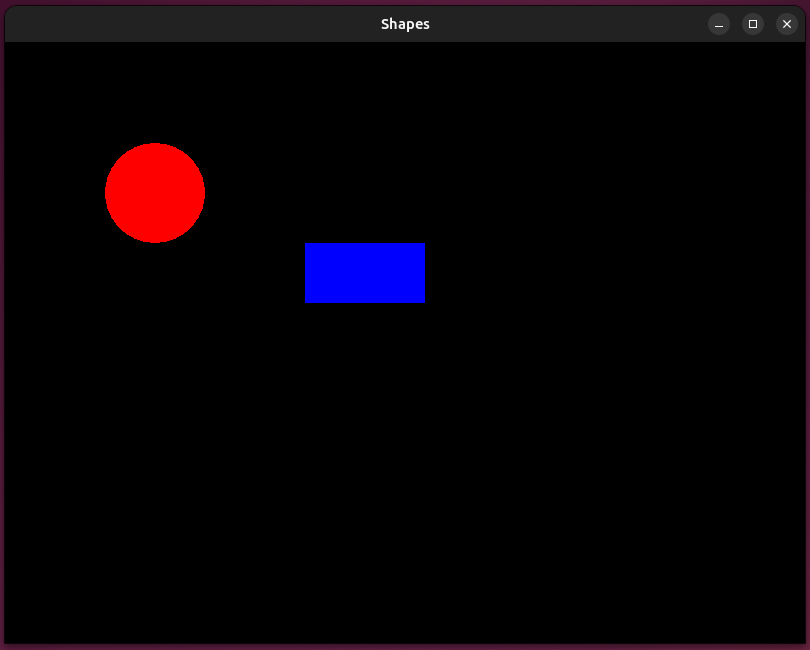
\includegraphics[width=0.8\textwidth]{src/img/sfml_shapes.png}
    \caption{Shapes}
    \label{fig:shapes}
\end{figure}

Рассмотрим обработку событий чуть подробнее. Пока запущено окно, оно постоянно проверяет было ли совершено какое-либо событие (нажатие клавиши, движение мыши и другие), если такое событие нашлось, то оно помещяется в очередь событий. Затем методом \texttt{pollEvent(event)} для окна мы вытаскиваем событие из очереди и присваиваем его переменной \texttt{event} класса \texttt{sf::Event}. После чего обрабатываем его и переходим к  следующему событию в случае, если очередь не пуста. Рассмотрим на примере движения мыши и нажатия клавиши \texttt{Escape}:

\begin{lstlisting}[style=myStyle]
if (event.type == sf::Event::KeyPressed) {
    if (event.key.code == sf::Keyboard::Escape)
        window.close();
}

if (event.type == sf::Event::MouseMoved) {
    std::cout << "Mouse position: " << event.mouseMove.x << ", " << event.mouseMove.y << std::endl;
}
\end{lstlisting}

Предварительно подключив заголовочный файл \texttt{iostream}, в результате получим, что при движении мыши в терминале будет обновляться её позиция, а по нажатию клавиши \texttt{Escape} программа завершится. Полный код (\autoref{lst:events}) и резульат (\autoref{fig:events}).
\begin{figure}[H]
    \centering
    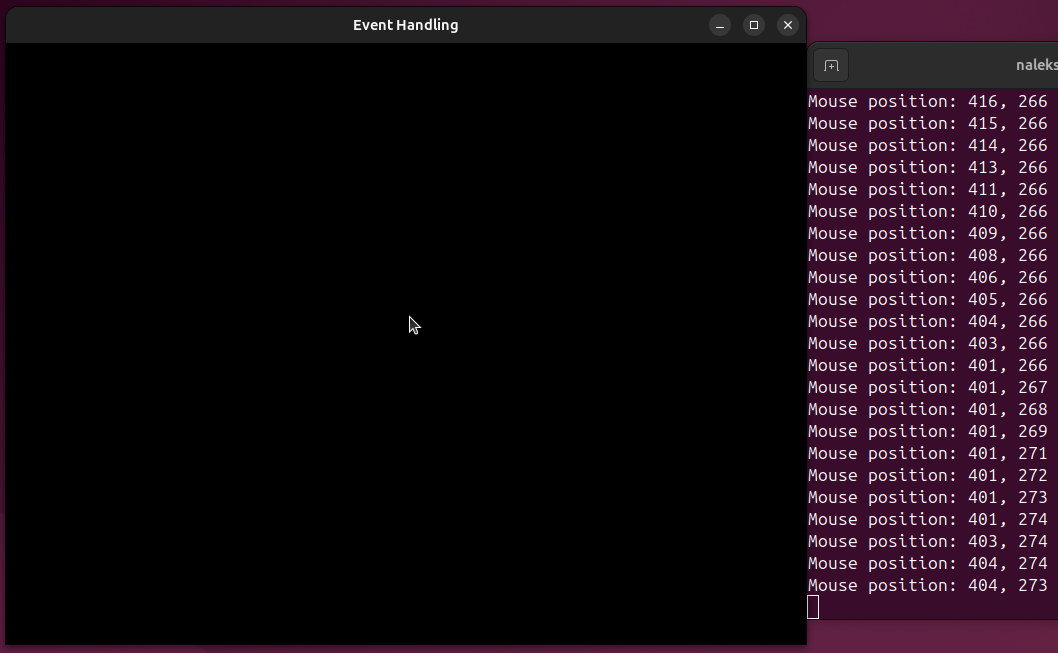
\includegraphics[width=0.8\textwidth]{src/img/sfml_events.png}
    \caption{Events}
    \label{fig:events}
\end{figure}

Последнее, что хотелось бы рассмотреть "--- это движение спрайта. В качестве последнего будет выступать круг, который мы уже умеем инициализировать и отображать. Реализуем самый простой способ движения "--- каждый кадр будем смещать спрайт на \texttt{X} и \texttt{Y} пикселей с помощью метода \texttt{move(X, Y)}. Для этого инициализируем нужные переменные и в основном цикле сдвинем спрайт:

\begin{lstlisting}[style=myStyle]
float speedX = 2.5f, speedY = 2.f;
ball.move(speedX, speedY);
\end{lstlisting}

Для того, чтобы постоянно в кадре наблюдать движение спрайта, пропишем простую логику. Пускай круг будет \flqq отскакивать\frqq\ от границ окна:

\begin{lstlisting}[style=myStyle]
if (ball.getPosition().x <= 0 || ball.getPosition().x >= 800 - 60) speedX = -speedX;
if (ball.getPosition().y <= 0 || ball.getPosition().y >= 600 - 60) speedY = -speedY;
\end{lstlisting}

Теперь мы можем постоянно наблюдать, как круг движется и \flqq ударяется\frqq\ о границы окна. На \autoref{fig:animation} светлым цветом показана текущая позиция круга, а на тёмных "--- позиции, которые он прошёл. В итоге движение получилось неидальным. Чтобы его улучшить (сделать более плавным) можно ограничить частоту кадров методом \texttt{setFramerateLimit()} для окна, а самый главный способ "--- преобразовать скорость из значения за кадр в значение, не зависящее от частоты кадров в секунду (\autoref{lst:animation}).
\begin{figure}[H]
    \centering
    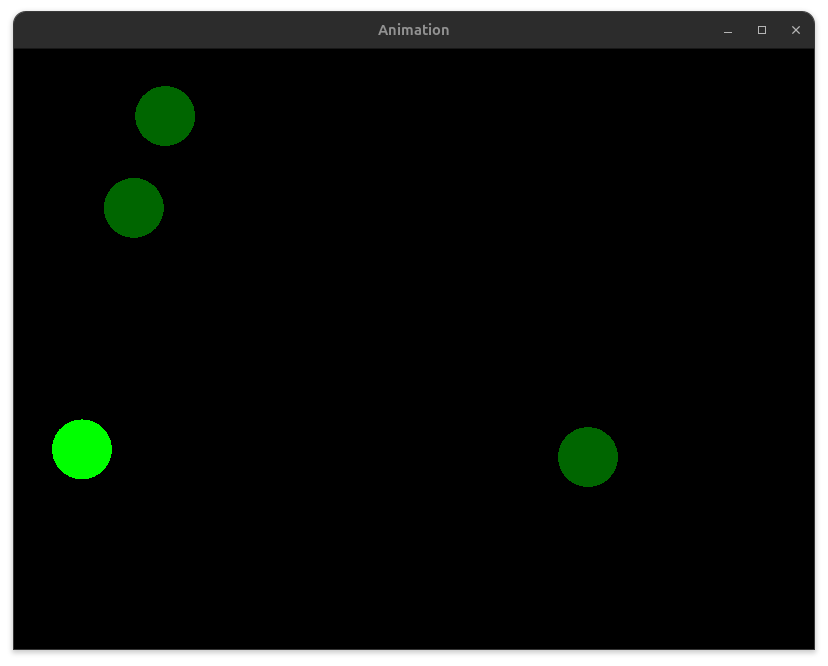
\includegraphics[width=0.8\textwidth]{src/img/sfml_animation.png}
    \caption{Animation}
    \label{fig:animation}
\end{figure}

\section{Реализация графических алгоритмов}
\subsection{Алгоритмы растеризации}
Алгоритм Брезенхэма для рисования линии "--- это алгоритм, определяющий, какие точки n"=мерного растра нужно закрасить, чтобы получить близкое приближение прямой линии между двумя заданными точками. Реализация алгоритма на C++\cite{bresenham}:
\begin{lstlisting}[style=myStyle]
void drawLine(int x1, int y1, int x2, int y2) {
    const int deltaX = abs(x2 - x1);
    const int deltaY = abs(y2 - y1);
    const int signX = x1 < x2 ? 1 : -1;
    const int signY = y1 < y2 ? 1 : -1;
    int error = deltaX - deltaY;
    setPixel(x2, y2);
    while (x1 != x2 || y1 != y2) {
        setPixel(x1, y1);
        int error2 = error * 2;
        if (error2 > -deltaY) {
            error -= deltaY;
            x1 -= signX;
        }
        if (error2 < deltaX) {
            error += deltaX;
            y1 -= signY;
        }
    }
}
\end{lstlisting}

Также существует алгоритм Брезенхэма для окружностей. По методу построения он похож на рисование линии. Строится дуга окружности для первого квадранта, а координаты точек окружности для остальных квадрантов получаются симметрично. На каждом шаге алгоритма рассматриваются три пикселя, из них выбирается наиболее подходящий путём сравнения расстояний от центра до выбранного пикселя с радиусом окружности. Реализация на C++\cite{bresenham}:
\begin{lstlisting}[style=myStyle]
void drawCircle(int x0, int y0, int radius) {
    int x = 0;
    int y = radius;
    int delta = 1 - 2 * radius;
    int error = 0;
    while (y >= 0) {
        setPixel(x0 + x, y0 + y);
        setPixel(x0 + x, y0 - y);
        setPixel(x0 - x, y0 + y);
        setPixel(x0 - x, y0 - y);
        error = 2 * (delta + y) - 1;
        if (delta < 0 && error <= 0) {
            ++x;
            delta += 2 * x + 1;
            continue;
        }
        if (delta >= 0 && error > 0) {
            --y;
            delta += 1 - 2 * y;
            continue;
        }
        ++x;
        delta += 2 * (x - y);
        --y;
    }
}
\end{lstlisting}
\subsection{Оптимизация графики}
\textbf{FPS} (Frames Per Second) "--- это количество кадров в секунду, которое отображается на экране во время воспроизведения видео или игры. Показатель FPS отражает, насколько плавно воспринимается изображение глазом пользователя. Чем выше значение FPS, тем более плавным и комфортным выглядит движение на экране.

Особенно важную роль FPS играет в играх. Так, FPS в играх "--- это показатель, который указывает, сколько кадров рендерится и отображается на экране за одну секунду. Благодаря высокому показателю FPS, картинка в играх является более плавной и приятной глазу. Однако, всё не так линейно, и здесь есть нюансы. Так, важен не только сам показатель в игре, но и его стабильное поддерживание. На устройстве или в игре в процессе может возникнуть проблема, из"=за которой FPS может резко снизиться. Если ошибки происходят периодически, то это гораздо хуже сказывается на качестве игры, чем низкий, но стабильный FPS.

Немаловажную роль в поддержке FPS играют показатели самой техники, то есть мониторов, с которых происходит воспроизведение. Частота обновления экрана оказывает сильное влияние на то, как быстро будет обновляться картинка. Например, частота экрана в 60 Гц способна менять кадр каждый 16 миллисекунд, а в 144 Гц "--- каждые 6 миллисекунд.

Разумеется, такое понятие, как FPS применяется и в съемке кино. Самая распространённая частота кадров в фильмах "--- это 24 FPS. Именно данный показатель является самым комфортным для зрителя при просмотре фильма. Показатель FPS в 24 единицы поддерживает реалистичность и плавность повествования, так как именно с такой частотой видят наши глаза в повседневной жизни. Усиленная плавность может казаться \flqq фальшивой\frqq\, так как в такой ситуации в сцене мы замечаем гораздо больше элементов, чем могли бы сделать это в реальности. Также у такой низкой частоты есть и практическая цель: съемка и монтаж видео с более высокой частотой кадров требуют больше места и производительности.

Если в случае с играми, плавность играет очень важную роль для поддержания качества игры и мгновенной отдачи действия игрока, то главная задача FPS в фильмах "--- это поддержание реалистичности кадра и сохранения художественного стиля.

\textbf{Двойная буферизация} "--- это метод рендеринга, при котором используются два буфера (то есть области памяти) для отображения графики. \textbf{Передний буфер} (front buffer) "--- отображается на экране, \textbf{задний буфер} (back buffer) "--- используется для рендеринга следующего кадра. После завершения рендеринга кадра в заднем буфере происходит обмен: задний буфер становится передним, передний буфер, в свою очередь, становится задним для следующего цикла рендеринга.

Преимущества двойной буферизации:
\begin{itemize}
    \item плавность анимации, так как кадры отображаются целиком, что очень важно для игр и интерактивных приложений;
    \item без двойной буферизации обновление экрана может происходить во время рендеринга, из-за чего может быть частичное отображение кадров.
\end{itemize}

Недостатки:
\begin{itemize}
    \item используется в 2 раза больше видеопамяти;
    \item возникают задержки, если рендеринг кадра занимает больше времени, чем период обновления монитора, частота кадров падает.
\end{itemize}

\textbf{Вертикальная синхронизация} (V"=Sync) "--- это технология, предназначенная для синхронизации частоты обновления монитора с частотой кадров, которую генерирует видеокарта. Основная цель V"=Sync "--- устранить разрывы изображения, которые могут возникать, когда видеокарта выводит кадры быстрее, чем монитор может их отображать.

Когда видеокарта генерирует кадры быстрее, чем монитор может их отображать, происходит разрыв изображения. Это означает, что на экране одновременно отображаются части нескольких кадров, что приводит к визуальным артефактам. V"=Sync решает эту проблему, заставляя видеокарту ждать, пока монитор не будет готов к отображению следующего кадра. Это достигается путем синхронизации частоты обновления монитора с частотой кадров видеокарты. Например, если монитор обновляется с частотой 60 Гц, V"=Sync заставляет видеокарту генерировать кадры с частотой не более 60 FPS, что предотвращает разрывы изображения.

Преимущества вертикальной синхронизации:
\begin{itemize}
    \item устранение разрывов изображения, что делает игровой процесс более плавным и приятным для глаз;
    \item помогает поддерживать стабильную частоту кадров, что может быть полезно в играх, где важна плавность и стабильность.
\end{itemize}

Недостатки:
\begin{itemize}
    \item Задержка ввода (input lag) может быть критична в динамических играх, она к тому, что действия игрока будут отображаться на экране с небольшим запозданием, что может повлиять на игровой процесс;
    \item в некоторых случаях может приводить к падению производительности, особенно если видеокарта не может поддерживать стабильную частоту кадров, равную частоте обновления монитора.
\end{itemize}

\conclusion
C++ играет важную роль в компьютерной графике благодаря производительности, низкоуровневому управлению ресурсами и интеграции с графическими библиотеками, такими как: SFML, OpenGL, SDL. На примерах реализации алгоритмов Брезенхэма, матричных преобразований и оптимизационных методов (двойная буферизация, V-Sync) показано, как язык обеспечивает контроль над рендерингом и аппаратными возможностями.

Использование C++ позволяет напрямую применять математические модели (цветовые пространства, координатные системы) в коде, что используется в задачах визуализации. На примере библиотеки SFML можно сделать вывод о стабильности FPS за счёт эффективного управления памятью и событиями.

Перспективные направления, например трассировка лучей, VR/AR, требуют ещё большей оптимизации, где C++ незаменим благодаря поддержке параллельных вычислений и низкоуровневых API.

% Отобразить все источники. Даже те, на которые нет ссылок.
% \nocite{*}

\bibliographystyle{ugost2003.bst}
\bibliography{thesis}

% Окончание основного документа и начало приложений Каждая последующая секция
% документа будет являться приложением
\appendix

\section{}
\lstinputlisting[style=myStyle, frame=single, rulecolor=\color{blue!30}, caption=Shapes, captionpos=b, label=lst:shapes]{src/codes/1.txt}

\lstinputlisting[style=myStyle, frame=single, rulecolor=\color{blue!30}, caption=Events, captionpos=b, label=lst:events]{src/codes/2.txt}

\lstinputlisting[style=myStyle, frame=single, rulecolor=\color{blue!30}, caption=Animation, captionpos=b, label=lst:animation]{src/codes/3.txt}

\end{document}
